\subsubsection{Registro de Usuarios}

El registro de Usuarios será mediante un formulario con el nombre, el email y la razón del registrante, y solamente el usuario administrador será capaz de aceptar o rechazar la solicitud de registro, para lo cual se implementó en la aplicación el \emph{formulario de registro} y el menú de \emph{menú de registros}. \\



\begin{description}
  \item[Formulario de Registro:] Para completar esta tarea se implementó en la vista de la aplicación el formulario, ver la figura \ref{fig:registro_form} usando \emph{ember-paper}, que como ya se mencionó es la librería usada para implementar la vista de la aplicación dandole el ``look and feel'' de una aplicación móvil. \\

  \begin{figure}[H]
        \begin{center}
          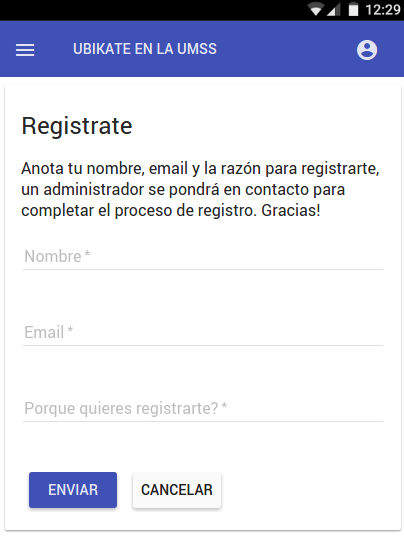
\includegraphics[width=0.5\textwidth]{registro_form}

          \caption{Formulario para Registro de Usuario}
          \label{fig:registro_form}
          \caption*{Fuente: Elaboración propia.}
        \end{center}
  \end{figure}


  Posteriormente se implementó en el \emph{backend} de la aplicación el módulo para guardar la solicitud de registro, para lo cual se  añadió el \emph{endpoint} en el API que escuche la petición POST generada al aceptar el \emph{formulario de registro}, este \emph{endpoint} inserta los datos colectados por el navegador en la base de datos para que estén disponibles posteriormente en el \emph{Menú de Registros}.\\


  \item[Menú de Registros] El \emph{menú de registro} será donde un usuario administrador puede ver todas las solicitudes de registro, y de acuerdo de la \emph{razón} de registro se puede determinar si la solicitud es de parte de un usuario responsable, en caso de necesitar más información del registrante se puede usar el \emph{email} enviado, una vez que el administrador considera que el registrante no va a jugar en el sistema para asegurar la integridad de la misma, puede \emph{aceptar} el registro, de esta forma el usuario recibirá un email donde se confirma el registro al sistema.\\





\end{description}


\subsubsection{Generación del Reporte}

Para la implementación del módulo que genere un reporte, se tuvo que modificar la tabla de los lugares, para saber cuántas veces un ``lugar'' es buscado, con esta informacion se puede proporcionar un reporte de frecuencia, para tal efecto se usó \emph{ember-charts}, que como se puede observar en el codigo \ref{chart_template}, sólo se necesita una línea para crear el reporte de frecuencia de la figura \ref{fig:reporte} \\

\begin{center}
  \begin{lstlisting}[label=chart_template,caption=Componente de \emph{Ember-charts}.]

{{horizontal-bar-chart data=model selectedSeedColor="green" sortAscending=false}}

  \end{lstlisting}
\end{center}

\begin{figure}[H]
      \begin{center}
        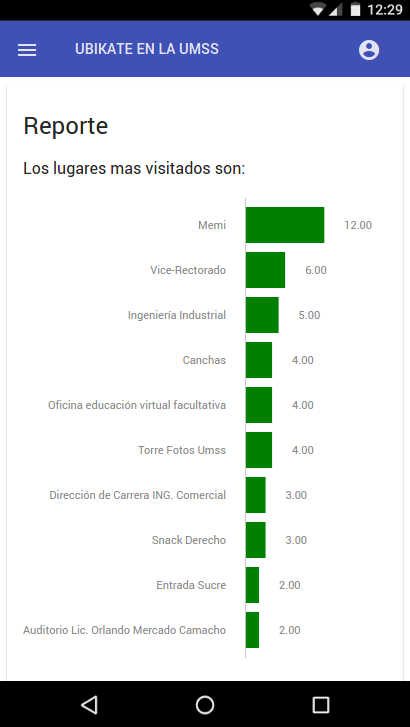
\includegraphics[width=0.5\textwidth]{reporte}

        \caption{Reporte de Frecuencia}
        \label{fig:reporte}
        \caption*{Fuente: Elaboración propia.}
      \end{center}
\end{figure}



Este reporte se obtiene al conocer la cantidad de veces que los usuarios han buscado un ``lugar'' mediante el SQL query, que se puede ver en el codigo \ref , el cual discrimina los primeros 10 lugares mas buscados dentro del campus universitario, ya que al existir tantas aulas y oficinas el reporte se haría muy extenso. \\

\begin{center}
  \begin{lstlisting}[label=request_visited,caption=Insertar un ``lugar'' en la base de datos.]

    router.get('places/visited/count',  (req, res) => {
      Place.forge()
        .where('visit_count', '>', '1')
        .orderBy('visit_count', 'DESC')
        .query((qb) => qb.limit(10))
        .fetchAll({columns: ["name as label", "visit_count as value"]})
        .then((visited) => {
            res.json(visited.toJSON());
        })
        .catch((err) => {
            res.status(500);
        });
    });

  \end{lstlisting}
\end{center}
